%% Influence Miner paper - results version (ACM acmart format).
%% Populated with the full run of Influence Miner (heuristic-v2, run 3) over the
%% DeMaP Miner Python corpus, 12 September 2026.
%% Compile with:  pdflatex influence-miner-acm-results.tex  (acmart.cls in the same folder)
%% For review submission: \documentclass[manuscript,screen,review,anonymous]{acmart}

\documentclass[sigconf,screen]{acmart}

\AtBeginDocument{%
  \providecommand\BibTeX{{Bib\TeX}}}

\usepackage{booktabs}
\usepackage{pgfplots}
\pgfplotsset{compat=1.18}

%% Draft metadata. Replace with the official ACM rights block after acceptance.
\setcopyright{none}
\copyrightyear{2026}
\acmYear{2026}
\acmDOI{}
\acmConference[Draft]{Draft manuscript prepared using the ACM acmart template}{September 2026}{New Zealand}
\acmISBN{}
\settopmatter{printacmref=false}

\begin{document}

\title[Influence Miner]{Influence Miner: Mining Strategic, Operational, Functional, and External Influence in Open Source Software Decision-Making}

\author{Pankaj Sharma}
\affiliation{%
  \institution{Universal College of Learning (UCOL)}
  \city{Palmerston North}
  \country{New Zealand}}

\renewcommand{\shortauthors}{Sharma}

\begin{abstract}
Open source software communities make consequential technical and governance decisions through distributed public discussions. Prior work has mined decision-making processes, rationales, preferences, sentiment and role prominence from such discussions, but the fine-grained mechanisms through which participants influence proposal outcomes have received less attention. This paper presents \emph{Influence Miner}, a tool-supported framework for identifying, classifying and analysing influence signals in open source decision-making discussions, and reports its first application to Python. Building on DeMaP Miner, Rationale Miner and Preference Miner, Influence Miner classifies sentence-level influence signals into thirteen mechanisms---strategic, operational, functional, tactical, authority, compatibility, security, standards, ecosystem, economic, organizational, coalition and user demand---and annotates each with a direction (supporting, blocking, revising), a scope (internal, external), a target, the author's role, and its temporal position relative to the proposal's decision. Applied to 523 Python Enhancement Proposals and 80,634 human-authored mailing-list messages (1999--2018), the heuristic prototype extracted 199,409 candidate influence sentences from 2,376 participants. Operational (27\%), functional (25\%), ecosystem (20\%) and compatibility (14\%) mechanisms dominate; functional and strategic arguments concentrate early and in the decision window while compatibility and operational arguments rise after the decision; influence signalling itself concentrates sharply in the four weeks around the decision; extending the corpus to September~2026 (780 PEPs, 291,100 candidates) shows that the community's mechanisms barely changed after the 2018 governance transition but that the Steering Council is a larger textual presence than the BDFL was and invokes authority four times as often; rejected proposals attract proportionally more functional, authority and tactical signals and fewer compatibility signals than accepted ones; and the direction of individual sentences barely discriminates outcomes, which supports the view that influence is not a matter of volume. Only 1.6\% of influence sentences coincide with Preference Miner's preference sentences, confirming that the two tools capture different phenomena. We also document two data-quality problems in the shared corpus that any tool built on it must handle. The contribution is a taxonomy, an open pipeline that produces annotation-ready output, and a first empirical baseline against which validated classifiers and a planned Bitcoin comparison can be measured.
\end{abstract}

\begin{CCSXML}
<ccs2012>
 <concept>
  <concept_id>10011007.10011006.10011050</concept_id>
  <concept_desc>Software and its engineering~Open source model</concept_desc>
  <concept_significance>500</concept_significance>
 </concept>
 <concept>
  <concept_id>10003120.10003121</concept_id>
  <concept_desc>Human-centered computing~Collaborative and social computing</concept_desc>
  <concept_significance>300</concept_significance>
 </concept>
 <concept>
  <concept_id>10002951.10003260.10003261</concept_id>
  <concept_desc>Information systems~Data mining</concept_desc>
  <concept_significance>300</concept_significance>
 </concept>
</ccs2012>
\end{CCSXML}

\ccsdesc[500]{Software and its engineering~Open source model}
\ccsdesc[300]{Human-centered computing~Collaborative and social computing}
\ccsdesc[300]{Information systems~Data mining}

\keywords{open source software, decision-making, influence mining, governance, Python Enhancement Proposals, Bitcoin Improvement Proposals, mailing lists, software repository mining}

\maketitle

\section{Introduction}

Open source software (OSS) development is often described as open, distributed and meritocratic. However, the openness of participation does not mean that all participants exert equal influence over decisions. Major design, governance and implementation decisions are shaped through public discussions, technical arguments, role-based authority, community norms, compatibility concerns, security concerns, ecosystem pressure and sometimes economic or organizational interests.

Proposal systems such as Python Enhancement Proposals (PEPs) and Bitcoin Improvement Proposals (BIPs) provide a valuable empirical setting for studying these dynamics. In Python, PEPs are design documents that propose major new features, collect community input and document design decisions. PEP authors are expected to build consensus and document dissenting opinions \cite{pep1}. Python's governance also changed historically from Guido van Rossum's BDFL authority to an elected Steering Council model, making it a useful project for studying how influence operates under changing governance arrangements \cite{pep13}.

Bitcoin offers a contrasting case. Its BIP repository serves as a publication medium and archive, but publication of a BIP does not indicate that a proposal has community consensus or is about to be adopted \cite{bitcoinbips}. BIP process documentation links some status changes to public discussion and rough consensus on the Bitcoin Development Mailing List \cite{bip3}. Influence in Bitcoin is therefore not reducible to formal titles or repository status; it must be traced through proposal discussions, objections, implementation signals, ecosystem uptake and community consensus-building.

Prior work has shown that OSS decision-making processes and rationales can be mined from public archives. Rationale Miner extracted rationale behind Python decisions from email archives and proposed a heuristics-based system for identifying decision rationales \cite{sharma2021rationale,sharma2024rationale}. Related work on Python examined how OSS roles influence decision-making across PEPs and email discussions \cite{sharma2021roles}. Bitcoin governance work has treated mailing-list and IRC traces as empirical sources for understanding influence mechanisms in permissionless blockchain communities \cite{thapa2021bitcoin}.

An important gap remains: we still need a systematic way to identify \emph{how influence is exercised in the text of decision-making discussions}. Existing process-mining and rationale-mining approaches can identify what decision processes occurred and why a decision may have been made, but they do not explain the mechanisms by which participants persuade, block, legitimise, redirect, reframe or operationalise proposals. Influence Miner addresses this gap.

This paper makes four contributions. First, it proposes a taxonomy of thirteen influence mechanisms in OSS decision-making. Second, it presents Influence Miner, an implemented extension of the DeMaP Miner tool family that extracts, classifies, scores and aggregates influence signals from proposal-linked mailing-list discussions and exports annotation-ready output. Third, it reports the first empirical application of the tool to the Python PEP corpus held by DeMaP Miner---523 proposals and 80,634 human-authored messages up to 2018, extended to 780 proposals and 114,388 messages up to September~2026 for the governance-era comparison---and answers five research questions with descriptive results. Fourth, it documents two data-quality problems in the shared corpus (shifted sender columns and automated senders) that materially distort actor-level results if left untreated, and shows how they were handled.

The results in this paper are produced by a transparent, rule-based prototype whose labels have not yet been validated against a gold standard. They are therefore reported as a baseline and as evidence that the pipeline works at scale, not as final measurements of influence in Python.

\section{Background and Motivation}

This study is positioned within the broader DeMaP Miner research agenda. DeMaP Miner originally focused on mining decision-making processes in OSS communities \cite{sharma2022demap}. Rationale Miner then extended this by extracting rationale behind decisions \cite{sharma2024rationale}. Preference Miner was proposed to identify whose preferences matter in OSS decisions by detecting approval, disapproval, favourable positions, unfavourable positions, elite contributor preferences and possible links between expressed preferences and proposal outcomes. Sentiment Miner was proposed to detect positive, negative and neutral sentiment, stress, toxicity and governance-era changes in community health.

Influence Miner complements these tools. While Preference Miner asks \emph{whose preferences matter}, Influence Miner asks \emph{how those preferences, arguments, roles and signals shape decisions}. Influence is not merely volume of participation. A participant who sends many emails may not influence a proposal, while another participant may send one message that reframes the problem, identifies a critical compatibility issue, invokes project authority or causes a proposal to be revised. Influence Miner therefore treats influence as a discursive, social, technical and governance phenomenon and aims to detect the sentence-level signals through which participants affect proposal trajectories.

\section{Research Questions}

The aim of this study is to develop and evaluate Influence Miner, a computational framework for mining influence mechanisms in OSS decision-making discussions.

\textbf{RQ1: What influence mechanisms appear in open source proposal discussions?} Which types of influence signals are used by participants, how frequently, and at which points of a proposal's life?

\textbf{RQ2: Which actors exercise influence, and through what mechanisms?} Is influence concentrated among formal leaders, core developers, proposal authors or the wider community, and do roles differ in the mechanisms they use?

\textbf{RQ3: How do influence mechanisms differ across governance models?} Within Python, do the discussions that continued after the 2018 governance transition differ from those under the BDFL model? (The Python--Bitcoin comparison is designed here but left for the next study.)

\textbf{RQ4: Do influence patterns align with proposal outcomes?} Are influence types and directions associated with acceptance, rejection, withdrawal or deferral?

\textbf{RQ5: How does Influence Miner complement existing decision-mining tools?}\  How much do influence signals overlap with the preference signals extracted by Preference Miner from the same corpus?

\section{Conceptualising Influence in OSS Decision-Making}

Influence is defined in this paper as a communicative or structural act that changes, constrains, legitimises, accelerates, blocks, reframes or redirects a proposal's decision trajectory. The unit of extraction in the prototype is the sentence; the unit of interpretation may be a message, a thread, an actor or a proposal trajectory.

Influence is different from preference. A preference expresses a position, such as support or opposition. Influence is the capacity of that position, argument, role or signal to affect the discussion or decision. A message may state a strong preference but fail to influence the proposal; conversely, a measured technical objection may substantially redirect the decision.

Influence is also different from sentiment. A message may be negative or frustrated without being influential, and a calm technical objection may be highly influential if it exposes a fundamental compatibility or security problem.

Influence is also different from rationale. A rationale explains why a decision was made. Influence Miner focuses on the mechanisms through which that rationale becomes accepted, contested or transformed during discussion. Influence Miner therefore sits between argument mining \cite{argumentMining}, rationale mining and social-network analysis: it connects what was said, who said it, when it was said and whether it appears to matter for the proposal trajectory.

\section{Influence Taxonomy}

Table~\ref{tab:taxonomy} summarises the taxonomy used by Influence Miner. It was developed from the DeMaP Miner research agenda, prior work on roles and rationale in Python, Bitcoin governance research \cite{thapa2021bitcoin}, and manual reading of PEP discussions. The thirteen types are not mutually exclusive: a sentence can carry several mechanisms at once, so the detector is multi-label. Table~\ref{tab:samples} in Section~\ref{sec:results} shows two sentences per mechanism as extracted by the tool.

\begin{table*}
\caption{Influence Miner taxonomy and indicative signals.}
\label{tab:taxonomy}
\begin{tabular}{p{0.16\textwidth}p{0.36\textwidth}p{0.40\textwidth}}
\toprule
\textbf{Influence type} & \textbf{Meaning} & \textbf{Indicative signals} \\
\midrule
Strategic & Shapes long-term direction, identity, philosophy or governance & future direction, project principles, Zen of Python, decentralisation, readability, simplicity \\
Operational & Shapes feasibility of implementation, maintenance, release, deployment, migration or testing & implementation burden, reference implementation, maintenance cost, release timing, documentation, backport \\
Functional & Shapes whether the proposed feature or protocol solves the intended problem & use case, edge case, API behaviour, semantics, syntax, alternative design, problem fit \\
Tactical & Shapes the immediate discussion trajectory & summarising, reframing, requesting evidence, compromise, deferral, closure, separate proposal \\
Authority & Uses formal or informal status to legitimise or block a decision & BDFL, delegate, steering council, BIP editor, core developer, pronouncement, veto \\
Compatibility & Shapes decisions through breaking-change and interoperability concerns & backward compatibility, existing code, Python 2/3, deprecation, old nodes, soft/hard fork \\
Security & Shapes decisions through safety, risk, attack, privacy or robustness concerns & vulnerability, attack surface, consensus failure, privacy, denial of service, crash \\
Standards & Uses existing standards, specifications or conventions as decision criteria & RFC, specification, PEP~8, protocol standard, compliance, convention \\
Ecosystem & Uses downstream adoption and ecosystem impact as decision criteria & PyPI, standard library, third-party packages, libraries, wallets, exchanges, miners, clients \\
Economic & Uses incentives, cost, funding, fees or business impact & cost, fees, funding, commercial pressure, developer time, block reward \\
Organizational & Uses companies, foundations, teams, working groups or institutions & PSF, company-backed maintainer, release team, committee, sponsor \\
Coalition & Uses collective alignment or repeated agreement as cumulative pressure & broad support, several developers, ``as others have said'', unanimous, seconded \\
User demand & Uses user needs, confusion, requests or adoption pressure & users want, beginners struggle, common request, pain point, widely used \\
\bottomrule
\end{tabular}
\end{table*}

\subsection{The Thirteen Mechanisms}

\emph{Strategic} influence shapes the long-term direction, identity or governance of the project (project philosophy, simplicity, readability, decentralisation, who has authority to decide). \emph{Operational} influence concerns implementation, maintenance, release management, testing, migration and coordination, and often determines whether an attractive proposal becomes feasible. \emph{Functional} influence concerns whether the proposed feature actually solves the intended problem (alternative designs, edge cases, complexity versus benefit). \emph{Tactical} influence covers short-term moves that shape a debate---summarising, reframing, narrowing scope, requesting evidence, proposing compromise, calling for a decision---and does not depend on formal authority. \emph{Authority} influence occurs when a participant's formal or informal status gives weight to a claim (BDFL, Steering Council, delegates, core developers, BIP editors, recognised experts); the tool records the role so that later analysis can test whether such statements are taken up, rather than assuming they are. \emph{Compatibility} influence covers backward compatibility, interoperability, migration and breaking changes, which can be decisive in mature ecosystems. \emph{Security} influence covers risk, vulnerability, attack surface, consensus failure, privacy and robustness; a single security objection can be decisive. \emph{Standards} influence relies on existing specifications and conventions. \emph{Ecosystem} influence rests on the needs of external projects, libraries, wallets, exchanges, miners or downstream communities. \emph{Economic} influence rests on incentives, cost, funding, fees or business interests. \emph{Organizational} influence comes from companies, foundations, teams or working groups. \emph{Coalition} influence arises when several participants visibly align. \emph{User-demand} influence connects decisions to what users need, request or struggle with.

\subsection{Internal and External Influence}

Orthogonally to the mechanism, Influence Miner records whether a signal is \emph{internal} (from or invoking the project's recognised governance and development structure) or \emph{external} (from or invoking users, downstream projects, companies, standards bodies, miners or market conditions), or \emph{mixed}, such as a core developer invoking user demand. This distinction is central to the planned Python--Bitcoin comparison: Python is expected to show stronger internal role-based influence, Bitcoin stronger ecosystem, economic, security and deployment-based influence.

\section{Influence Miner: Implementation}

Influence Miner is implemented as a Java extension of DeMaP Miner, following the design of Preference Miner, and reads the same MySQL corpus. Figure~\ref{fig:pipeline} shows the pipeline; this section describes what was built.

\begin{figure*}
  \centering
  \fbox{%
    \begin{minipage}{0.92\textwidth}
    \centering
    proposal-linked messages $\rightarrow$ automated-sender filter $\rightarrow$ identity and role resolution $\rightarrow$ text cleaning and sentence splitting $\rightarrow$ multi-label influence classification (type, direction, scope, target) $\rightarrow$ outcome and temporal features $\rightarrow$ heuristic scoring $\rightarrow$ candidate table $\rightarrow$ actor/proposal aggregation $\rightarrow$ CSV, annotation sample, report
    \end{minipage}}
  \caption{Influence Miner pipeline as implemented.}
  \Description{A flow diagram showing proposal-linked messages flowing through filtering, identity resolution, cleaning, classification, feature computation, scoring, storage, aggregation and reporting.}
  \label{fig:pipeline}
\end{figure*}

\subsection{Data Source and Message Filtering}

Messages are read from DeMaP Miner's \texttt{allmessages} table, which links mailing-list messages to PEP numbers by explicit references and subject matching \cite{sharma2022demap}. Column names are discovered at run time so that the same code can be pointed at a BIP database. Two classes of messages are excluded because they carry no human discussion: commit notifications from \texttt{python-checkins} (which embed entire PEP texts and would otherwise account for the majority of extracted sentences) and the bug- and patch-tracker robots (\texttt{report@bugs.python.org}, \texttt{noreply@sourceforge.net}). The exclusion lists are configurable. Messages that mention several PEPs appear once per PEP; duplicates within a PEP are collapsed.

\subsection{Identity and Role Resolution}

Actor identity is the person, not the address. The corpus provides a clustered display name and a pre-computed role per message; for the rows imported by a newer loader (chiefly 2017--2018, including the whole PEP~572 discussion) we found that the sender-address columns are shifted by one row---they belong to the \emph{next} message---while the clustered name and role agree with the raw ``From:'' header stored with the message body (Section~\ref{sec:threats}). Influence Miner detects these rows, keeps the name and role, and takes the address from the raw header. Roles are then resolved in layers: an optional manual, time-bounded mapping file; the role recorded on the message (BDFL, BDFL delegate, core developer, PEP editor, community member); proposal-specific roles from PEP metadata (proposal author, BDFL delegate); project-wide tables of core developers and PEP editors with their appointment dates; and well-known identities. Proposal-specific roles take precedence over project-wide ones, following the corpus's own convention, except that the BDFL keeps that role. Actors are keyed by the clustered name, which merges one person's several addresses.

\subsection{Text Cleaning and Sentence Splitting}

Each message body is cleaned before splitting: quoted lines, ``On \ldots wrote:'' introductions, forwarded header blocks, message-id and address debris, signature blocks, mailing-list footers, embedded PEP text attachments, code, diffs and tracebacks are removed, and URLs are replaced by a placeholder. Sentences are split on terminal punctuation with protection for abbreviations, version numbers and proposal references; short vote lines such as ``+1'' and ``$-$1'' are kept as sentences. A noise filter drops fragments shorter than three words, sentences longer than 120 words and lines that are mostly non-alphabetic. Cleaning is deliberately conservative: the research depends on real discussion content.

\subsection{Classification}

Four rule-based detectors label each sentence. The \emph{type} detector matches cue phrases for the thirteen mechanisms on word boundaries, accepts British and American spellings, requires disambiguating context for broad words (``break'' only near compatibility vocabulary, ``risk'' only near security vocabulary, ``team'' only near release or core vocabulary), and records the cue phrases that fired as \emph{evidence}, so that every label can be traced. The \emph{direction} detector is conservative: it classifies a sentence as supporting or blocking only on explicit stance phrases or votes, resolves negations (``I don't object'' is supporting, ``I can't support'' is blocking), treats a sentence with both supporting and blocking cues as ambiguous, demotes hedged sentences and questions, and otherwise assigns revising (revise, defer, clarify, narrow, alternative, compromise \ldots) or neutral. The \emph{scope} detector combines the author's role with actor words in the sentence; role alone never yields ``external''. The \emph{target} detector assigns governance, implementation, security, compatibility, ecosystem, users or proposal.

\subsection{Outcome, Temporal Features and Scoring}

The proposal outcome is resolved from the corpus's table of accepted and rejected PEPs and, for the remaining PEPs, from the PEP state history mined from the PEP repository log, normalised to accepted, rejected, withdrawn, deferred, final, active, superseded, draft, provisional or unknown, with the decision timestamp. From the decision date and the PEP creation date the tool computes the number of days between the message and the decision and a coarse decision phase (pre-draft, early discussion, active debate, revision, decision window, post-decision). A configurable governance split date (default 12~July~2018, when Guido van Rossum stepped down) assigns each message to the BDFL or post-BDFL era. Direction is compared with outcome to obtain an \emph{alignment} flag: supporting signals align with accepted, final or active proposals; blocking with rejected, withdrawn or deferred ones; revising with deferred, superseded, draft or provisional ones.

A transparent additive score combines the number of mechanisms detected, deontic and decision language, justification language, explicit reference to the proposal, a non-neutral direction, a resolved scope and target, the author's formal role, and proximity to the decision (only when the decision date is known and the message precedes it), with penalties for hedging and very short sentences. Sentences scoring at least 1.0 are stored as candidates with all labels, evidence cues, role, outcome and temporal features.

\subsection{Aggregation and Outputs}

A batch runner processes one proposal, a range or the whole corpus, continues after errors and logs per-proposal statistics. An aggregator populates per-actor and per-proposal summary tables and computes multi-label type distributions, direction, scope, role, phase and era distributions, type-by-outcome and type-by-era cross-tabulations and alignment counts. An exporter writes these as CSV files; a sampler exports a stratified annotation sheet (top-scored, random, per-type and per-outcome strata) with empty human-label columns; and a report generator writes a plain-text summary. All code, SQL and configuration are in the DeMaP Miner repository.

\section{Study Design}

\subsection{Corpus}

The study uses the DeMaP Miner Python corpus \cite{sharma2022demap,sharma2024rationale}: messages from the python-dev, python-ideas, python-list, python-3000, distutils-sig, python-committers and python-announce lists, linked to PEP numbers, spanning May~1999 to November~2018. Table~\ref{tab:corpus} summarises the run. Of the 109,046 PEP-linked message rows, 28,412 were excluded as automated senders, leaving 80,634 human-authored messages across 523 PEPs. Cleaning and splitting produced 999,943 sentences, of which 199,409 (19.9\%) carried at least one influence mechanism and scored above the threshold. The run took 31~minutes on a laptop.

\begin{table}[t]
\caption{Corpus and extraction summary.}
\label{tab:corpus}
\begin{tabular}{lr}
\toprule
PEPs with linked messages & 523 \\
PEP-linked message rows & 109,046 \\
\quad automated (commit/tracker) rows excluded & 28,412 \\
\quad human-authored messages processed & 80,634 \\
Sentences after cleaning & 999,943 \\
Influence candidate sentences stored & 199,409 \\
PEPs with at least one candidate & 508 \\
Distinct participants (actors) & 2,376 \\
Period covered & 1999-05 to 2018-11 \\
\bottomrule
\end{tabular}
\end{table}

Outcomes were resolved for 479 of the 523 PEPs: 151 accepted, 94 rejected, 83 final, 42 withdrawn, 34 draft, 30 deferred, 25 active and 5 superseded; 44 PEPs (1,343 candidates, 0.7\%) have no recorded state. Candidates on accepted or final proposals make up 64\% of the corpus, rejected 12\%, withdrawn 7\% and deferred 4\%.


\paragraph{Steering Council era extension.} For RQ3 the corpus was extended to September~2026. Mailing-list archives were downloaded from mail.python.org (Mailman~2 monthly files, and Mailman~3 mbox exports converted to the same format) for python-dev, python-ideas, python-committers, python-list, python-checkins and python-bugs-list; the discussions that moved to discuss.python.org were collected through its JSON API for the PEPs, Ideas, Core Development and Committers categories (3,685 topics, 63,714 posts) and rewritten as pipermail-style messages so that DeMaP Miner's own reader links them to PEPs. PEP metadata and the complete status history (1,859 status changes to 739 PEPs) were regenerated from the git history of the \texttt{python/peps} repository, which also covers the older PEPs consistently. Roles were extended with a \emph{steering council} label from the election results in PEPs 8100--8107 and with the current core-team roster and its join/leave dates. The extension adds 289,000 messages, 41,000 of them PEP-linked, and raises the corpus to 780 PEPs with 114,388 human-authored PEP-linked messages; the full Influence Miner run over it yields 291,100 candidates from 3,613 participants. Sections~\ref{sec:results}.1, .2, .4 and .5 report the original 1999--2018 corpus; Section~\ref{sec:results}.3 uses the extended one.
\subsection{Analysis}

RQ1 is answered by the multi-label type distribution, its profile across decision phases and the timing of signals relative to the decision. RQ2 uses the role distribution, actor-level aggregates and direction by role. RQ3 compares mechanism, role, direction and alignment distributions of BDFL-era and Steering-Council-era candidates on the extended corpus, and the mechanism mix of the decision-makers of each era (the BDFL; Steering Council members during their terms). RQ4 compares type distributions across outcomes, per-proposal averages, and direction--outcome alignment against the base rate. RQ5 compares influence sentences with the 12,690 sentences stored by Preference Miner for the same PEPs after normalising whitespace and punctuation. All statistics are descriptive; no causal claim is made.

\section{Results}
\label{sec:results}

\subsection{RQ1: Influence Mechanisms}

Table~\ref{tab:rq1} shows how often each mechanism occurs among the 199,409 candidates. Because a sentence can carry several mechanisms, the percentages sum to more than 100 (on average 1.27 mechanisms per candidate). Four mechanisms dominate: operational (27.1\%), functional (25.2\%), ecosystem (19.9\%) and compatibility (14.4\%). Standards signals (9.8\%) are inflated by the many references to PEP~8 and PEP~257 as style standards. Authority signals appear in 7.1\% of candidates, strategic signals in 5.0\% and tactical moves in 4.9\%. The mechanisms that the Bitcoin literature emphasises---economic (2.3\%), coalition (2.0\%) and security (2.8\%)---are rare in Python's language-design discussions, as expected.

\begin{table}[t]
\caption{RQ1: influence mechanisms in 199,409 candidate sentences (multi-label).}
\label{tab:rq1}
\begin{tabular}{lrr}
\toprule
Mechanism & Candidates & \% of candidates \\
\midrule
Operational & 54,098 & 27.1 \\
Functional & 50,233 & 25.2 \\
Ecosystem & 39,593 & 19.9 \\
Compatibility & 28,656 & 14.4 \\
Standards & 19,631 & 9.8 \\
Authority & 14,078 & 7.1 \\
Strategic & 10,018 & 5.0 \\
Tactical & 9,780 & 4.9 \\
User demand & 7,193 & 3.6 \\
Organizational & 5,914 & 3.0 \\
Security & 5,529 & 2.8 \\
Economic & 4,555 & 2.3 \\
Coalition & 4,010 & 2.0 \\
\bottomrule
\end{tabular}
\end{table}

Table~\ref{tab:samples} shows two sentences per mechanism as the tool extracted and labelled them, chosen among high-scoring candidates with different roles and directions. They illustrate what the labels mean in practice: the BDFL closing a debate (``I heard all the feedback \ldots and have decided''), a delegate asking whether a PEP is ready for pronouncement, a core developer proposing that a contentious part be deferred to a separate PEP, a proposal author conceding a cost, a community member reporting classroom evidence.

\begin{table*}
\caption{Sample statements per influence mechanism, as extracted and labelled by Influence Miner (role and direction as assigned by the tool; ``rev.'' = revising).}
\label{tab:samples}
\small
\begin{tabular}{p{0.095\textwidth}p{0.045\textwidth}p{0.125\textwidth}p{0.66\textwidth}}
\toprule
\textbf{Mechanism} & \textbf{Dir.} & \textbf{Role, PEP} & \textbf{Sentence} \\
\midrule
Strategic & supp. & core dev., 492 & In principle, I support the PEP, on the basis that working towards better coroutine/async support in Python seems worthwhile to me. \\
 & block. & core dev., 20 & I'm not putting either version forward as paragons of Pythonic code, but honestly, they're not so awful that we should reject this PEP because of the risk that somebody will do this. \\
\midrule
Operational & supp. & BDFL, 3147 & I'm fine with the implementation going in and the PEP being marked as accepted as long as you get to the clarifications I suggest below soon after. \\
 & rev. & BDFL, 365 & Unless I find someone besides Phillip who is interested in having this included and is willing to help maintain it, I don't really think it would be wise to accept this into the standard library. \\
\midrule
Functional & supp. & BDFL, 435 & I heard all the feedback, took into account my own thoughts, and have decided that we should go ahead with this syntax and the \_getframe() hack. \\
 & rev. & BDFL, 525 & The provisional status is because this is a big project and it's likely that we'll need to tweak some small aspect of the API once the code is in, even after 3.6.0 is out. \\
\midrule
Tactical & rev. & core dev., 565 & IMHO the core of the PEP 565 is to propose a compromise to separate ``own code'' and ``external code'' (cannot be modified). \\
 & rev. & core dev., 470 & Instead, the PEP should highlight this compromise and defer it to a separate PEP. \\
\midrule
Authority & rev. & BDFL, 441 & So is the PEP ready for pronouncement or should there be more discussion? \\
 & neutral & BDFL, 380 & I just can't get used to this aspect of PEP 3152, so I'm rejecting it. Sorry Greg, but that's the end. \\
\midrule
Compatibility & supp. & core dev., 476 & So while I agree with the intent of PEP 476, and like the suggested end state, I'm back to thinking that the transition plan for existing corporate users needs more work before it can be accepted. \\
 & block. & author, 438 & However, I think PEP470 needs to achieve stronger backward compatibility for end-users because, as is typical for the 99\%, they like to see change but hate to be forced to change themselves. \\
\midrule
Security & rev. & author, 438 & If projects host on HTTP instead of HTTPS, users are vulnerable against MITM attacks whereas PEP438f provides a checksummed link from PyPI which cannot be easily man-in-the-middled. \\
 & rev. & author, 504 & The PEP would then stay deferred until someone actually did the research and demonstrated a practical attack. \\
\midrule
Standards & supp. & core dev., 371 & I agree that the threading and the pyprocessing APIs should be PEP 8 compliant, but I think 2 APIs is almost worse than one wrong one. \\
 & neutral & delegate, 427 & The compatibility tag spec itself looks fine to me, so with the above clarifications, I will accept the PEP. \\
\midrule
Ecosystem & supp. & core dev., 470 & Since PyPI is legally run by the PSF, the PSF board will have to approve the new terms. \\
 & rev. & BDFL, 365 & If its inclusion is really meant just as a bootstrap to simplify installing other package management solutions, as the PEP claims, I would prefer to see something with a much smaller footprint. \\
\midrule
Economic & neutral & author, 441 & IMO, the costs aren't worth the benefits, and I'd like to remove this proposal and simply document that applications packed up with pyzaa need to be tested to ensure they work from a zipfile. \\
 & rev. & community, 285 & Probably `should', at least---yet more work (`transitional', to be sure), and so yet another cost of the PEP's adoption. \\
\midrule
Organizational & neutral & BDFL, 3149 & That's about as large a committee I'd be comfortable to appoint for any specific PEP. \\
 & rev. & core dev., 466 & Presumably the need for such enhancements is there (or there'd be no need for this PEP) so is it simply that companies like Red Hat don't know that they have this option? \\
\midrule
Coalition & supp. & BDFL, 3154 & Assuming Tim doesn't object (hi Tim!) I think this PEP is fine to accept---all the ideas sound good, and I agree with moving to support 8-byte sizes and framing. \\
 & neutral & BDFL, 363 & This seems to be the overwhelming feedback at this point, so I'm withdrawing my support for the proposal. \\
\midrule
User demand & rev. & core dev., 362 & Since this will be an error that beginners see (frequently), I suggest ArgumentError is more friendly than BindError. \\
 & rev. & community, 572 & I've only had the chance to test the proposal on $\sim$20 students so far, but I'd like the chance to gather more data for your consideration before the PEP is accepted or rejected. \\
\bottomrule
\end{tabular}
\end{table*}

Direction is neutral for 88.1\% of candidates; 8.6\% are revising, 2.0\% supporting and 1.3\% blocking. This is by design: the detector only commits to a direction on explicit cues, so the non-neutral 11.9\% are high-precision signals for later analysis. Scope is internal for 61.7\%, mixed for 4.5\%, external for 2.5\% and unresolved for 31.3\%.

\paragraph{When influence is exercised.} Temporally, 33.3\% of candidates were written \emph{after} the recorded decision (implementation and follow-up discussion), 33.1\% during active debate, 9.5\% in the first month after the PEP was created, 8.1\% in the two weeks before the decision and 6.2\% in the preceding revision window. Figure~\ref{fig:timeline} shows the volume of influence signals per two-week bin relative to the decision date: signalling builds up over the preceding quarter and peaks sharply in the two weeks before the decision (13,702 candidates) and the two weeks after it (9,022), then falls back within a month to the pre-decision level. Sentences with an explicit stance follow the same curve (604 in the last two weeks). The decision moment recorded in the PEP repository is therefore also the moment of maximum argumentative activity in the mailing lists, which supports the use of the decision date to define the ``decision window'' phase.

\begin{figure}[t]
\centering
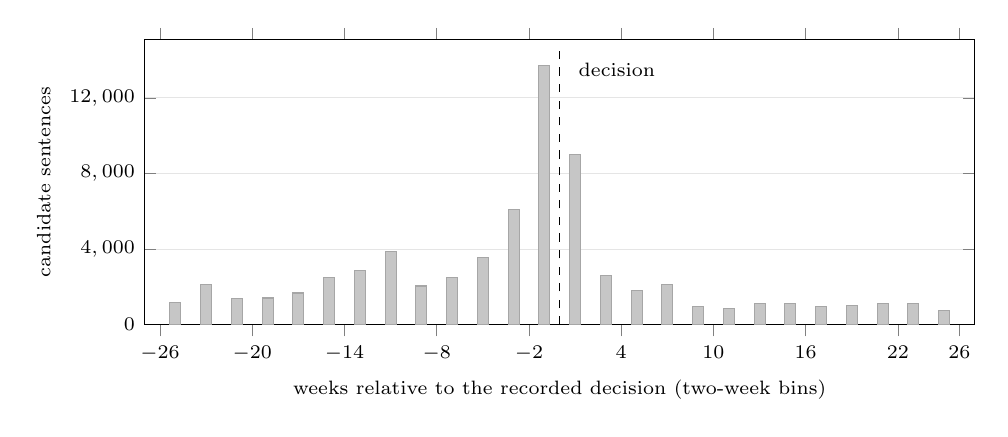
\begin{tikzpicture}
\begin{axis}[
  width=\columnwidth, height=5.2cm,
  ybar, bar width=4pt,
  xlabel={weeks relative to the recorded decision (two-week bins)},
  ylabel={candidate sentences},
  xmin=-27, xmax=27, ymin=0,
  xtick={-26,-20,-14,-8,-2,4,10,16,22,26},
  scaled y ticks=false,
  ytick={0,4000,8000,12000},
  yticklabel style={/pgf/number format/fixed, /pgf/number format/1000 sep={,}},
  tick label style={font=\scriptsize}, label style={font=\scriptsize},
  enlarge x limits=false,
  ymajorgrids, grid style={gray!20},
]
\addplot[fill=gray!45, draw=gray!70] coordinates {
(-25,1187) (-23,2130) (-21,1362) (-19,1413) (-17,1677) (-15,2486) (-13,2887) (-11,3883) (-9,2045) (-7,2512) (-5,3559) (-3,6115) (-1,13702)
(1,9022) (3,2618) (5,1788) (7,2114) (9,947) (11,837) (13,1138) (15,1124) (17,975) (19,1025) (21,1108) (23,1098) (25,758) };
\draw[dashed] (axis cs:0,0) -- (axis cs:0,14500);
\node[font=\scriptsize, anchor=west] at (axis cs:0.6,13500) {decision};
\end{axis}
\end{tikzpicture}
\caption{Influence candidates per two-week bin relative to the proposal's recorded decision date (69,510 candidates within $\pm$26 weeks of a known decision).}
\Description{Bar chart of candidate sentences per two-week bin from 26 weeks before to 26 weeks after the decision; volume rises slowly, peaks at 13,702 in the two weeks before the decision and 9,022 in the two weeks after, then drops to around one to two thousand per bin.}
\label{fig:timeline}
\end{figure}

\paragraph{Which mechanisms when.} Figure~\ref{fig:phases} profiles the mechanisms across four phases of a proposal's life. Functional arguments are most frequent early (30.1\% of early-discussion candidates) and again in the decision window (29.0\%), when the community is deciding whether the proposal solves the right problem; strategic arguments follow the same shape (6.8\% early, 6.2\% in the window, 3.9\% after). Compatibility (11.1\% $\rightarrow$ 17.8\%) and operational arguments (24.0\% $\rightarrow$ 30.2\%) rise steadily and dominate \emph{after} the decision, when accepted proposals are implemented and their effects on existing code are discovered. Authority, tactical and coalition signals are flat or fall after the decision. Influence Miner thus recovers the expected lifecycle of a design decision from the text alone: what-and-why arguments first, how-and-what-breaks arguments later.

\begin{figure*}[t]
\centering
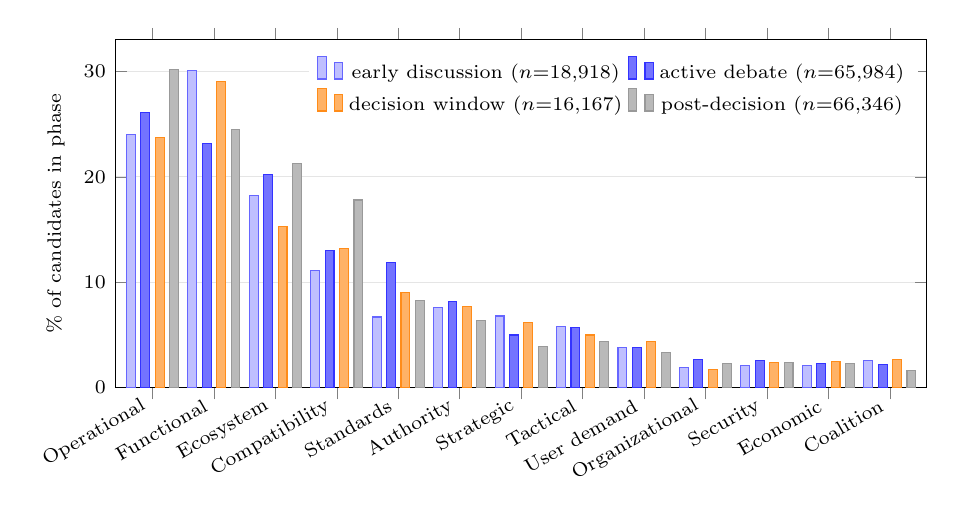
\begin{tikzpicture}
\begin{axis}[
  width=0.98\textwidth, height=6cm,
  ybar, bar width=3.2pt,
  ylabel={\% of candidates in phase},
  ymin=0, ymax=33,
  symbolic x coords={Operational,Functional,Ecosystem,Compatibility,Standards,Authority,Strategic,Tactical,User demand,Organizational,Security,Economic,Coalition},
  xtick=data, x tick label style={rotate=30, anchor=east, font=\scriptsize},
  tick label style={font=\scriptsize}, label style={font=\scriptsize},
  enlarge x limits=0.05,
  legend style={font=\scriptsize, at={(0.99,0.97)}, anchor=north east, legend columns=2, draw=none, fill=white},
  ymajorgrids, grid style={gray!20},
]
\addplot[fill=blue!25, draw=blue!60] coordinates {(Operational,24.0) (Functional,30.1) (Ecosystem,18.2) (Compatibility,11.1) (Standards,6.7) (Authority,7.6) (Strategic,6.8) (Tactical,5.8) (User demand,3.8) (Organizational,1.9) (Security,2.1) (Economic,2.1) (Coalition,2.6)};
\addplot[fill=blue!55, draw=blue!80] coordinates {(Operational,26.1) (Functional,23.2) (Ecosystem,20.2) (Compatibility,13.0) (Standards,11.9) (Authority,8.2) (Strategic,5.0) (Tactical,5.7) (User demand,3.8) (Organizational,2.7) (Security,2.6) (Economic,2.3) (Coalition,2.2)};
\addplot[fill=orange!60, draw=orange!90] coordinates {(Operational,23.7) (Functional,29.0) (Ecosystem,15.3) (Compatibility,13.2) (Standards,9.0) (Authority,7.7) (Strategic,6.2) (Tactical,5.0) (User demand,4.4) (Organizational,1.7) (Security,2.4) (Economic,2.5) (Coalition,2.7)};
\addplot[fill=gray!55, draw=gray!80] coordinates {(Operational,30.2) (Functional,24.5) (Ecosystem,21.3) (Compatibility,17.8) (Standards,8.3) (Authority,6.4) (Strategic,3.9) (Tactical,4.4) (User demand,3.3) (Organizational,2.3) (Security,2.4) (Economic,2.3) (Coalition,1.6)};
\legend{{early discussion ($n$=18{,}918)},{active debate ($n$=65{,}984)},{decision window ($n$=16{,}167)},{post-decision ($n$=66{,}346)}}
\end{axis}
\end{tikzpicture}
\caption{Mechanism profile by decision phase (share of the phase's candidates carrying each mechanism; multi-label, so bars within a phase sum to more than 100\%).}
\Description{Grouped bar chart with thirteen mechanisms on the x axis and four bars per mechanism for early discussion, active debate, decision window and post-decision. Functional and strategic bars are highest early and in the decision window; compatibility and operational bars are highest after the decision.}
\label{fig:phases}
\end{figure*}

\subsection{RQ2: Who Exercises Influence}

Table~\ref{tab:rq2} breaks candidates down by the author's role on the proposal in question. Core developers produce 25.6\% of candidates and community members 36.6\%, but the 138 core developers identified are far fewer than the 2,162 community members, so influence signalling per person is much denser among core developers. Proposal authors contribute 15.7\% and the BDFL alone 10.9\% of all candidates (21,793 sentences across 464 PEPs). PEP editors (9.4\%) and BDFL delegates (1.7\%) are small groups with high per-person volume.

\begin{table}[t]
\caption{RQ2: candidates and participants by role. Roles are proposal-specific; a person is counted under the role they held most often.}
\label{tab:rq2}
\begin{tabular}{lrrr}
\toprule
Role & Candidates & \% & Participants \\
\midrule
Community member & 72,976 & 36.6 & 2,162 \\
Core developer & 51,026 & 25.6 & 138 \\
Proposal author & 31,369 & 15.7 & 52 \\
BDFL & 21,793 & 10.9 & 1 \\
PEP editor & 18,656 & 9.4 & 8 \\
BDFL delegate & 3,431 & 1.7 & 1 \\
Unknown & 158 & 0.1 & 12 \\
\bottomrule
\end{tabular}
\end{table}

The fifteen most active participants account for 52\% of all candidates: Guido van Rossum (24,336 candidates, 464 PEPs), Brett Cannon (16,342; 285), Nick Coghlan (16,040; 332), Steven Bethard (7,270; 95), Phillip Eby (5,202; 108), Victor Stinner (4,932; 142), Donald Stufft (4,188; 67), Paul Moore (4,186; 178), Ned Deily (3,671; 73), Steven D'Aprano (3,528; 151), Tony Meyer, Yury Selivanov, Barry Warsaw, Martin von L\"owis and Tim Peters. Their mechanism mix is remarkably uniform---operational, functional and ecosystem lead for almost all of them---with two exceptions: Donald Stufft's first mechanism is \emph{ecosystem} (packaging and PyPI) and Tim Peters's third is \emph{authority}.

Mechanism mix by role differs modestly, with one clear exception: PEP editors' candidates carry far more \emph{authority} (10.4\%) and \emph{tactical} (8.3\%) signals than any other role (core developers 5.0\% and 3.1\%), which reflects the editors' process work of asking whether a PEP is ready for pronouncement, calling for decisions and closing threads. The BDFL's own candidates carry the \emph{least} authority signalling of all roles (3.0\%) but the most organizational (5.6\%) and security (3.6\%) signals; the BDFL exercises authority rather than invoking it. Community members carry the most functional (21.6\%), strategic (4.8\%), user-demand (3.5\%) and coalition (2.0\%) signals. Direction by role is similar across roles: between 8.4\% (PEP editors) and 18.1\% (BDFL delegates) of each role's candidates carry a non-neutral direction, and blocking signals are between 0.8\% and 1.5\% for every role. Formal authority is therefore not visible as a larger share of explicit stance sentences; it is visible in \emph{what} those sentences do (pronouncements, acceptances), which Table~\ref{tab:samples} shows and which the annotation study will quantify.

\subsection{RQ3: Governance Eras}

Table~\ref{tab:rq3} compares mechanism shares under the BDFL model (1999--July~2018, 174,750 candidates on 494 PEPs from 2,310 participants) and under the Steering Council model (July~2018--September~2026, 100,778 candidates on 579 PEPs from 1,546 participants). The two eras are similar in outline: the same four mechanisms lead, and the direction profile is identical (1.4\% vs.\ 1.3\% blocking, 2.1\% vs.\ 2.0\% supporting, 8.9\% vs.\ 9.1\% revising). Within that outline the Steering Council era shifts towards \emph{functional} (25.4 $\rightarrow$ 28.9\%) and \emph{operational} (26.9 $\rightarrow$ 29.0\%) arguments and away from \emph{ecosystem} (20.0 $\rightarrow$ 16.7\%) and \emph{standards} (9.6 $\rightarrow$ 7.4\%) ones; \emph{authority} signals rise by a third (7.0 $\rightarrow$ 9.6\%) and \emph{organizational} signals by half (2.4 $\rightarrow$ 3.7\%). A preliminary analysis restricted to the four months after the transition had shown authority and strategic signals doubling; over the full era that spike, which coincides with the governance PEPs 8010--8016, flattens into a moderate and persistent increase.

\begin{table}[t]
\caption{RQ3: mechanism share (\%) by governance era, and mechanism mix of the decision-makers themselves.}
\label{tab:rq3}
\begin{tabular}{lrrcrr}
\toprule
 & \multicolumn{2}{c}{All candidates} & & \multicolumn{2}{c}{Decision-makers} \\
\cmidrule{2-3}\cmidrule{5-6}
Mechanism & BDFL era & SC era & & BDFL & SC members \\
 & 174,750 & 100,778 & & 28,301 & 17,581 \\
\midrule
Operational & 26.9 & 29.0 & & 21.8 & 31.5 \\
Functional & 25.4 & 28.9 & & 20.0 & 14.2 \\
Ecosystem & 20.0 & 16.7 & & 15.9 & 7.6 \\
Compatibility & 14.5 & 13.3 & & 10.3 & 15.1 \\
Standards & 9.6 & 7.4 & & 8.8 & 3.3 \\
Authority & 7.0 & 9.6 & & 3.0 & \textbf{11.9} \\
Strategic & 4.8 & 5.8 & & 3.7 & 1.7 \\
Tactical & 5.2 & 5.1 & & 2.5 & 3.6 \\
User demand & 3.8 & 3.8 & & 2.3 & 1.8 \\
Security & 2.6 & 2.4 & & 3.6 & 1.0 \\
Organizational & 2.4 & 3.7 & & 5.6 & 5.1 \\
Economic & 2.4 & 2.5 & & 1.3 & 2.1 \\
Coalition & 2.1 & 2.0 & & 1.2 & 1.1 \\
\bottomrule
\multicolumn{6}{l}{\footnotesize Decision-maker columns are multi-label hit shares; SC = Steering Council.}
\end{tabular}
\end{table}

The clearer change is \emph{who} carries the signals. Steering Council members author 12.1\% of the era's candidates, against 5.1\% for the BDFL and 1.9\% for BDFL delegates before (core developers 30.9\% vs.\ 27.9\%, community members 35.9\% vs.\ 40.5\%, proposal authors 14.4\% vs.\ 16.4\%). The council is therefore a larger textual presence in proposal discussions than the BDFL was, and it speaks differently (right-hand columns of Table~\ref{tab:rq3}): council members' candidates invoke \emph{authority} four times as often as the BDFL's (11.9\% vs.\ 3.0\%), and are dominated by \emph{operational} (31.5\%) and \emph{compatibility} (15.1\%) arguments, with far fewer \emph{functional} (14.2\% vs.\ 20.0\%), \emph{ecosystem} (7.6\% vs.\ 15.9\%) and \emph{strategic} (1.7\% vs.\ 3.7\%) ones. A body that decides by a documented process must refer to its decisions, deadlines and delegations; a single BDFL could simply pronounce. Design and vision arguments have correspondingly moved to proposal authors and the community. Direction--outcome alignment also changes: supporting sentences align with positive outcomes in 62.7\% of cases in the Steering Council era against 73.5\% before, and revising sentences align in 17.1\% against 6.3\%, because many recent proposals are still draft, provisional or deferred.

\subsection{RQ4: Alignment with Outcomes}

Table~\ref{tab:rq4} shows mechanism shares by final outcome. Compared with accepted PEPs, rejected PEPs attract proportionally more \emph{functional} (23.7\% vs.\ 19.9\%), \emph{authority} (6.2\% vs.\ 4.8\%) and \emph{tactical} (5.0\% vs.\ 3.5\%) signals and fewer \emph{compatibility} (8.7\% vs.\ 12.1\%), \emph{operational} (18.9\% vs.\ 21.6\%) and \emph{ecosystem} (14.9\% vs.\ 16.8\%) signals. Read together with Figure~\ref{fig:phases}, this says that accepted proposals accumulate the post-decision compatibility and implementation discussion that rejected ones never reach, whereas rejected proposals stay contested at the level of whether the feature solves a real problem and who gets to decide. Withdrawn and deferred proposals sit between the two.

\begin{table}[t]
\caption{RQ4: mechanism share (\%) by proposal outcome.}
\label{tab:rq4}
\begin{tabular}{lrrrr}
\toprule
Mechanism & Accepted & Rejected & Withdrawn & Deferred \\
 & (151 PEPs) & (94) & (42) & (30) \\
\midrule
Operational & 21.6 & 18.9 & 21.0 & 22.5 \\
Functional & 19.9 & 23.7 & 21.0 & 22.0 \\
Ecosystem & 16.8 & 14.9 & 17.0 & 16.2 \\
Compatibility & 12.1 & 8.7 & 11.0 & 8.0 \\
Standards & 7.0 & 6.5 & 7.8 & 6.5 \\
Authority & 4.8 & 6.2 & 4.4 & 5.1 \\
Strategic & 3.7 & 4.7 & 3.3 & 4.8 \\
Tactical & 3.5 & 5.0 & 3.7 & 4.1 \\
User demand & 3.0 & 3.0 & 2.4 & 2.4 \\
Security & 2.2 & 1.9 & 2.7 & 2.2 \\
Organizational & 2.0 & 2.6 & 2.4 & 2.6 \\
Economic & 1.9 & 2.1 & 1.9 & 2.0 \\
Coalition & 1.6 & 1.8 & 1.3 & 1.6 \\
\bottomrule
\end{tabular}
\end{table}

At the proposal level, accepted PEPs are discussed more (on average 613 candidates from 36 participants, versus 269 from 22 for rejected PEPs), and rejected PEPs have a slightly higher blocking share (1.6\% vs.\ 1.2\%) and a slightly lower supporting share (1.6\% vs.\ 1.9\%). These differences are small. Direction--outcome alignment makes the same point: 72.9\% of supporting sentences sit on proposals that were eventually accepted, final or active---but 72.4\% of \emph{all} candidates do, so the alignment is no better than the base rate; blocking sentences align with negative outcomes in 26.5\% of cases against a base rate of 23.8\%. Counting explicit stance sentences therefore does not predict outcomes. This is not a failure of the tool but a finding consistent with its premise: influence is exercised through arguments and roles rather than through the number of votes cast, and the interesting cases are those where the majority stance and the decision diverge.

\subsection{RQ5: Complementarity with Preference Miner}

Preference Miner stored 12,690 preference sentences for the same PEPs. Only 3,142 of them (24.8\%) are also influence candidates, and they represent 1.6\% of the influence candidates (Jaccard 0.015). The overlap consists of sentences that both state a stance and invoke a mechanism (``I support the PEP because it would break less existing code''). The two tools therefore look at largely different sentences: Preference Miner at stance-bearing sentences regardless of argument, Influence Miner at argument-bearing sentences regardless of stance. Combining them---for instance, following the preference trajectory of a participant whose influence signals are mostly compatibility objections---is the natural next step.

\section{Discussion}

\paragraph{What the mechanism profile says about Python.} Python's proposal discussions are dominated by operational, functional, ecosystem and compatibility arguments. Influence in a mature language community is exercised mainly by arguing about whether something can be implemented and maintained, whether it solves a real problem, what it does to the ecosystem and what it breaks---and the lifecycle profile shows these arguments arriving in that order. Explicit appeals to authority are comparatively rare (7\%) even though the BDFL is the single most active participant, which supports the position taken in Section~4 that authority should be measured by uptake rather than assumed from role.

\paragraph{Governance transition.} The era comparison is the first quantitative trace of the governance transition in the discussions themselves. The mechanisms the community uses barely changed; what changed is the decision-makers' share of the conversation and their register. A five-person council that must document, delegate and announce invokes authority four times as often as the BDFL did and argues about implementation and compatibility rather than design, while functional and strategic arguments moved to authors and the community. Whether this reflects the council's mandate (PEP~13 asks it to decide, not to design) or the maturity of the language is a question for the qualitative follow-up.

\paragraph{Volume is not influence.} The near-base-rate alignment of stance sentences with outcomes is the most important methodological result. It shows that a decision-mining tool that counted supporting and blocking sentences would learn nothing about outcomes in this corpus. Influence Miner's value lies in the mechanisms, roles and timing attached to each sentence, which allow the analyst to ask \emph{which} objections were taken up and \emph{whose} arguments the final PEP text reflects.

\paragraph{Data quality as a research finding.} Two problems in the shared corpus would have silently distorted every actor-level result: automated senders contributed most of the raw sentences, and the shifted sender columns would have credited PEP~572's discussion to the wrong people. Both are now handled in the tool and documented so that Rationale Miner and Preference Miner results built on the same rows can be re-checked.

\paragraph{Towards Bitcoin.} The taxonomy already contains the Bitcoin vocabulary (soft/hard forks, miners, wallets, consensus failure, fee market), the outcome resolver accepts BIP statuses, and the message source discovers column names, so the pipeline can be pointed at the DeMaP Miner BIP database. The comparison will test the expectation that Bitcoin shows stronger ecosystem, economic, security and deployment-based influence and weaker internal role-based influence.

\section{Threats to Validity}
\label{sec:threats}

\paragraph{Construct validity.} The labels are produced by cue phrases and have not been validated against human judgement; precision and recall are unknown. Table~\ref{tab:samples} was chosen to show the mechanisms clearly, but the same extraction also produces clear errors: a BDFL sentence reporting broad support (``I haven't seen substantial opposition against the PEP \ldots many people have explicitly posted in support of it'') is labelled \emph{blocking} because of the word ``opposition''; ``Google should not [be] needed to find a PEP'' fires the \emph{organizational} cue on a company name used as a verb; any mention of PEP~8 fires \emph{standards}. The stratified annotation sample exported by the tool (top-scored, random, per-mechanism and per-outcome strata) is the instrument for the two-coder study that must precede any stronger claim. Multi-label counts overstate the number of distinct arguments.

\paragraph{Internal validity.} Alignment between direction and outcome is descriptive association at sentence level; sentences from the same author and message are not independent, and no causal inference is attempted. A third of candidates post-date the recorded decision, so ``influence on the decision'' must be qualified by the decision phase, which the tool records.

\paragraph{Data quality.} Two problems were found in \texttt{allmessages}. First, rows imported by the newer loader (identifiable by a ``From \ldots'' sender field, mostly 2017--2018) carry the sender address of the \emph{next} row: checked against the raw ``From:'' header stored with the body, the clustered name agrees with the header for 9,532 of the 10,831 such rows but the address column for only 3,155. Identity is therefore taken from the name and the address from the header; an earlier version of the tool made the opposite assumption and mis-attributed the PEP~572 discussion. Second, 28,412 rows are commit notifications and tracker robots; the first full run that included them produced 565,952 candidates, 307,000 of them credited to a single committer because all commits share one address. Both problems are corrected, but other studies of this corpus should check for them.

\paragraph{External validity.} RQ1, RQ2, RQ4 and RQ5 are reported on the 1999--2018 mailing-list corpus; RQ3 adds the Steering Council era, whose discussions come partly from a different medium (Discourse threads, where usernames stand in for addresses and quoting conventions differ). Findings should not be generalised to projects with different governance structures until the Bitcoin comparison is done.

\paragraph{Role identification.} Roles are proposal-specific and partly time-sensitive (core developer and PEP editor appointment dates are used), but the corpus's own role labels are trusted where present; Steering Council membership is resolved by name and term, and Discourse participants are identified by username, so a person using different names on the two media would be counted twice.

\section{Conclusion}

This paper presented Influence Miner, a framework and implemented tool for mining influence mechanisms in OSS decision-making discussions, and its first application to the Python PEP corpus. Influence Miner extends DeMaP Miner, Rationale Miner and Preference Miner by classifying sentence-level influence signals into strategic, operational, functional, tactical, authority, compatibility, security, standards, ecosystem, economic, organizational, coalition and user-demand mechanisms, and by attaching direction, scope, target, role, outcome and timing to each signal. Across 523 PEPs and 80,634 messages, operational, functional, ecosystem and compatibility mechanisms dominate; functional and strategic arguments come first and compatibility and operational arguments follow the decision; signalling peaks in the four weeks around the decision; after the 2018 governance transition the mechanisms barely change but the Steering Council becomes a larger and more authority-invoking presence than the BDFL was; rejected proposals remain contested on functional and authority grounds while accepted ones move to compatibility and implementation; stance volume does not track outcomes; and influence and preference signals occupy largely different sentences. The next steps are the two-coder annotation study that the tool's sampler supports, replacement of the cue rules by validated classifiers, reply-uptake and revision-linkage features, a qualitative reading of the Steering Council era, and the Bitcoin comparison for which the pipeline is prepared.

\begin{thebibliography}{00}

\bibitem{pep1}
Python Software Foundation. 2026. PEP 1 -- PEP Purpose and Guidelines. Retrieved September 12, 2026 from \url{https://peps.python.org/pep-0001/}

\bibitem{pep13}
Python Software Foundation. 2026. PEP 13 -- Python Language Governance. Retrieved September 12, 2026 from \url{https://peps.python.org/pep-0013/}

\bibitem{bitcoinbips}
Bitcoin Core Contributors. 2026. Bitcoin Improvement Proposals repository. Retrieved September 12, 2026 from \url{https://github.com/bitcoin/bips}

\bibitem{bip3}
Bitcoin Core Contributors. 2026. BIP 3 -- Updated BIP Process. Retrieved September 12, 2026 from \url{https://github.com/bitcoin/bips/blob/master/bip-0003.md}

\bibitem{sharma2021rationale}
Pankajeshwara Nand Sharma, Bastin Tony Roy Savarimuthu, and Nigel Stanger. 2021. Extracting Rationale for Open Source Software Development Decisions -- A Study of Python Email Archives. \emph{arXiv:2102.05232}. \url{https://arxiv.org/abs/2102.05232}

\bibitem{sharma2024rationale}
Pankajeshwara Nand Sharma, Bastin Tony Roy Savarimuthu, and Nigel Stanger. 2024. How are decisions made in open source software communities? Uncovering rationale from Python email repositories. \emph{Journal of Software: Evolution and Process}. \url{https://doi.org/10.1002/smr.2526}

\bibitem{sharma2021roles}
Pankajeshwara Nand Sharma, Bastin Tony Roy Savarimuthu, and Nigel Stanger. 2021. Influence of Roles in Decision-Making during OSS Development -- A Study of Python. \emph{arXiv:2106.02209}. \url{https://arxiv.org/abs/2106.02209}

\bibitem{sharma2022demap}
Pankajeshwara Nand Sharma, Bastin Tony Roy Savarimuthu, and Nigel Stanger. 2022. Unearthing open source decision-making processes: A case study of Python Enhancement Proposals. \emph{Software: Practice and Experience}. \url{https://doi.org/10.1002/spe.3128}

\bibitem{thapa2021bitcoin}
Rewat Thapa, Pankajeshwara Sharma, Joschka Andreas H{\"u}llmann, and Bastin Tony Roy Savarimuthu. 2021. Identifying Influence Mechanisms in Permissionless Blockchain Communities: The Bitcoin Case. In \emph{Proceedings of the 42nd International Conference on Information Systems (ICIS 2021)}, 1--17.

\bibitem{rationaleDesign}
Antony Tang, Yan Jin, and Jun Han. 2007. A rationale-based architecture model for design traceability and reasoning. \emph{Journal of Systems and Software} 80, 6, 918--934.

\bibitem{argumentMining}
Raquel Mochales and Marie-Francine Moens. 2011. Argumentation mining. \emph{Artificial Intelligence and Law} 19, 1, 1--22.

\bibitem{ossGovernance}
Kevin Crowston, Kangning Wei, James Howison, and Andrea Wiggins. 2012. Free/Libre open-source software development: What we know and what we do not know. \emph{ACM Computing Surveys} 44, 2, Article 7.

\end{thebibliography}

\end{document}
